\documentclass[12pt,a4paper]{article}
\usepackage{fontspec}
\usepackage{xunicode}
\usepackage{csquotes}
\usepackage{enumitem}
%\usepackage{titling}
\usepackage{setspace}
\usepackage{xcolor}
\usepackage[french]{babel}
\usepackage[style=enc]{biblatex}
\usepackage{graphicx}
\usepackage{pythonhighlight}
\usepackage[hidelinks,linktoc=all]{hyperref}

\addbibresource{../bib_TAL.bib}
\graphicspath{ {../images/} }

\setlength{\parindent}{0pt}
\setlength\bibitemsep{1.5\itemsep}
\setlength{\footnotesep}{0.8\baselineskip}
\addtolength{\skip\footins}{1pc plus 5pt minus 3pt}

\renewcommand{\baselinestretch}{1.0} 


\begin{document}


%%%%%%%%%%%%%%%%%%%%%% DOCUMENT
		\begin{center}
			
			\bigskip
			
			\begin{large}				
				ÉCOLE NATIONALE DES CHARTES\\
				UNIVERSITÉ PARIS, SCIENCES \& LETTRES
			\end{large}
			\begin{center}\rule{2cm}{0.02cm}\end{center}
			
			\bigskip
			\bigskip
			\bigskip
			\begin{large}
				Francesco Paolo Savatteri\\
				\vspace{1.3\baselineskip}
				Avril 2024
			\end{large}
			%selon le cas
			
			\vspace{8\baselineskip}
			
		\setstretch{1.5}
		\begin{Large}
				\emph{Pre-processing} de données textuelles collectées de plusieurs sources: une approche fondée sur sentence-BERT et la réduction dimensionnelle
		\end{Large}
	
	
	
			\vfill
			
			
		\end{center}

	
	\thispagestyle{empty}	
	\cleardoublepage

\tableofcontents

\clearpage


\section{Introduction}
Lors de la création d'un dataset à partir de différentes sources, l'un des principaux problèmes consiste à rendre les données suffisamment homogènes - le niveau de suffisance dépendant des objectifs pour lesquels le dataset est construit. Dans le cas des données textuelles, cela s'applique non seulement à un certain nombre d'éléments quantitatifs ou facilement reconnaissables – longueur du texte, langue, etc. – mais aussi à leur propre signification.\\

 Les pages suivantes présentent une approche possible du \emph{pre-processing} des données textuelles collectées à partir de diverses sources, qui permet également de vérifier l'homogénéité du sens des textes contenus dans l'ensemble de données.\\
 
 Tout le code utilisé est disponible en ligne à cette adresse : \url{https://github.com/savaij/devoir_TAL}

\section{Les données}
Les données concernent le monde \emph{incel} italien. Les incels - abréviation de “involuntary celibates” - sont les membres d'une certaine communauté en ligne. Ils se caractérisent par le fait qu'il s'agit principalement d'hommes blancs hétérosexuels qui se décrivent comme incapables d'avoir un partenaire romantique ou sexuel bien qu'ils en aient envie.
\\

En particulier, les données ont été collectées à partir de trois sources différentes grâce à des techniques de \emph{data scraping}:
\begin{enumerate}[label= -]
\item groupe sur Telegram “Azione Incel”
\item groupe sur Telegram “FDB”
\item forum en ligne “il forum dei brutti”\footnote{”le forum des moches“ en italien}
\end{enumerate}

Les données sont donc constituées des messages postés sur les deux groupes télégrammes et des messages postés sur le forum.\\

Le dataset à partir duquel commence notre analyse est déjà le résultat de l'union des données de ces différentes sources et contient trois colonnes : id, text, file\_label. “id” est un code numérique que nous pouvons ignorer pour le moment. “text” est la chaîne de texte qui contient le contenu du message et “file\_label” est une étiquette qui indique la source d'où provient le texte.

\section{Le processus}
Le prétraitement de ces données est divisé en deux étapes principales. La première concerne des aspects plus simples : l'élimination des données nulles et la vérification de la longueur des textes en excluant les valeurs aberrantes. La seconde concerne le sens de ces textes, afin de vérifier l'homogénéité de leur contenu.
\\
\subsection{Première phase}


\section{Le contrôle}
Pour être sûrs que nos résultats sont fiables - et que ce n'est pas, par exemple, le modèle linguistique qui ne fonctionne pas - nous devons effectuer des tests de contrôle. Il s'agit essentiellement de comparer les textes Incel avec des textes qui n'ont rien à voir avec eux, pour comprendre comment cela affecte leur visualisation.\\

Dans ce cas, on a utilisé un jeu de données contenant des résumés d'articles du journal italien “ilpost”\footcite{ilpost2022}. Il a été créé par le \emph{Applied Recognition Technology Laboratory} (Arte-Lab), un laboratoire de recherché rattaché à l'Université de l'Insubrie (Varese, Italie). En particulier, on a utilisé la partie "train" du dataset, qui correspond 35.201 titres. À l'aide du même modèle sentence-BERT utilisé précédemment, on a créé des embedding. Ensuite, les embeddings que nous venons de créer ont été fusionnés avec ceux du jeu de données incel de départ et nous avons appliqué les techniques de réduction dimensionnelle mentionnées précédemment, PCA et UMAP. Les représentations graphiques des résultats sont présentées ci-dessous\footnote{Pour la représentation des points obtenus avec UMAP, une librairie graphique différente a été utilisée pour rendre la visualisation plus claire.}. Les points verts sont les phrases de contrôle et les points rouges sont les phrases incel.

\begin{figure}[h!]
	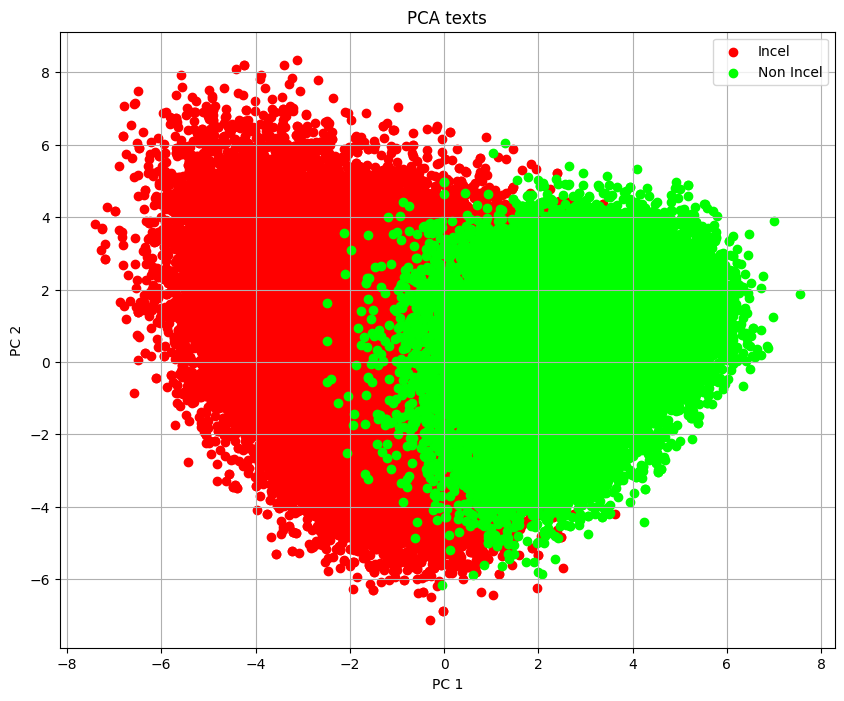
\includegraphics[scale=0.4]{PCA_test.png}
	\centering
	\caption{Plot des données réduites par PCA}
\end{figure}

\begin{figure}[h!]
	\includegraphics[scale=0.45]{umap_test.png}
	\centering
	\caption{Plot des données réduites par UMAP}
\end{figure}

\clearpage

Comme on peut le voir, les deux groupes peuvent être identifiés  assez facilement à partir des deux graphiques. 
Cela montre globalement que le modèle de langue utilisé fonctionne et que, par conséquent, le chevauchement presque complet des points dans les figures 1 et 2 peut être considéré comme une preuve de l'homogénéité du sens des phrases dans le dataset de départ.

\section{Les limites}
L'approche présentée dans ces pages est incomplète pour plusieurs raisons. \\ 
Tout d'abord, la méthode du groupe de contrôle décrite dans la section précédente n'est utile qu'à un niveau général et intuitif. Pour comparer les résultats de manière plus rigoureuse, il existe des méthodes mathématiques qui permettent de mesurer le niveau de \emph{clustering} des données. En outre, la performance d'un modèle sentence-BERT peut elle-même être calculée en utilisant des jeux de données déjà existants, même en italien, afin d'obtenir des scores précis. L'approche décrite dans ces pages n'est donc utile que pour une analyse préliminaire des données dans les cas où un niveau de précision particulièrement élevé n'est pas requis.\\

En outre, un autre aspect n'est pas pris en compte : la présence de valeurs aberrantes. Comme on peut le voir dans la figure 2, certains points sont très éloignés des autres (il y en a aussi dans le cas de la PCA, bien qu'ils ne soient pas visibles dans le graphique). Cela suggère qu'il pourrait s'agir de valeurs aberrantes. Une approche plus complète devrait identifier et décider comment traiter ces valeurs. Une méthode possible, par exemple, consiste à calculer un embedding moyen et à déterminer la distance de chaque texte par rapport à la moyenne, afin d'éliminer ensuite les valeurs trop élevées – la définition de “trop élevé” pouvant être trouvée de différentes manières. 

\newpage

\printbibliography
\end{document}